\textbf{Markov chain Monte Carlo} (\textit{MCMC}) algorithms work quite differently from rejection sampling or likelihood weighting. Instead of creating each time a 
new sample, MCMC algorithms generate each sample by making a random change to the preceding sample. It can be helpful to think of an MCMC algorithm as a set of worlds\footnote{All the several worlds are not \textit{atomic event} but only \textit{states}.},
where we are in a \textit{current state} specifying a value for every variable and generate a \textit{new state} by making random changes to the current state. \vspace{3.5pt}

Every sample defined in that way is meaningful, but how to do design them? To answer this query, we need to change something seen so far, and in this case we have to redefine
the way for drawing samples. \vspace{3.5pt}

Until now, every method studied suffers from one main problem: estimated distributions never converge to true distributions in the long run, expecially when many samples 
are generated. This last observation can be an useful hint for understanding the \textbf{Gibbs sampling}. \vspace{3.5pt}

Given the image shown below, the main idea of Gibbs sampling consists of drawing all the states which represent every single change for any non-evidence variable. As likelihood
sampling, evidence variables are fixed. \vspace{3.5pt}

Moving on, we suppose that our current state is:
\begin{center} \vspace{3.5pt}
    $\langle Cloudy=True, Sprinkler=True, Rain=False, WetGrass=True \rangle$.
\end{center} \vspace{3.5pt}
To make a new sample, the algorithm focuses on one non-evidence variable at a time, in this case $Rain$, and it generates a new related value. The next state will be the same if $Rain$
is again \textit{false}, or it would be 
\begin{center} \vspace{3.5pt}
    $\langle Cloudy=True, Sprinkler=True, Rain=True, WetGrass=True \rangle$
\end{center} \vspace{3.5pt}
if the sampled value is \textit{true}. \vspace{3.5pt}
\begin{center}
    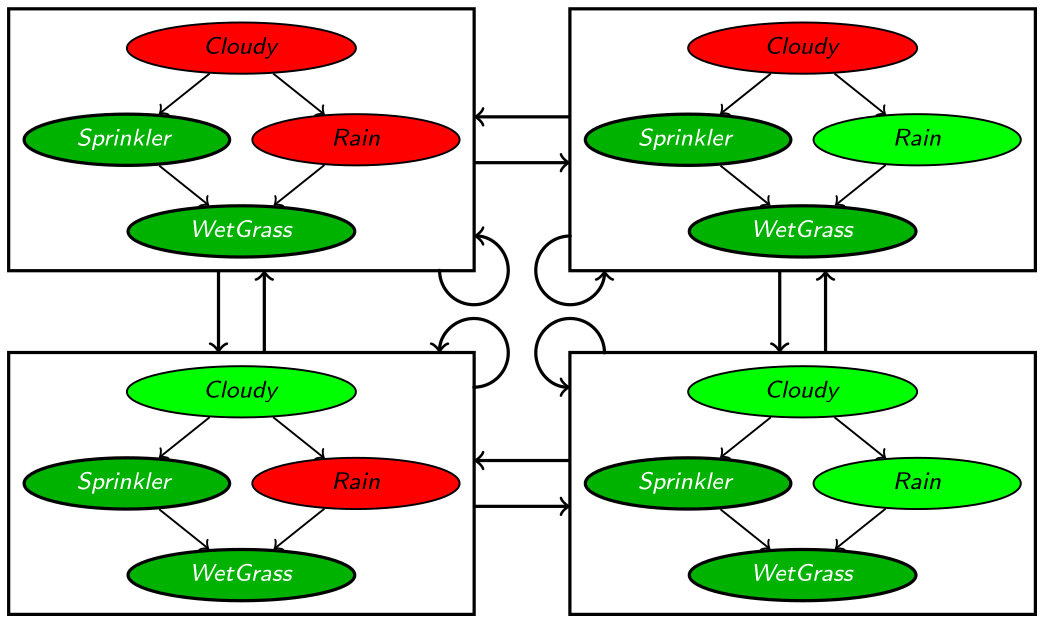
\includegraphics[width=0.7\textwidth]{img/img16.png}
\end{center} \vspace{3.5pt}
The sampling for the non-evidence variable $X_i$ is done by looking its \textit{Markov blanket}\footnote{Given a random variable $X_i$ its \textbf{Markov blanket}, $X_i$ is conditionally independent of all other nodes in the network.}.
Therefore, Gibbs method samples only the Markov blanket associated, without any time recompute all the random variables that composed the network. Probabilities given the Markov
blanket are calculated as follows: \vspace{3.5pt}
\begin{center}
    $P(x_i|mb(X_i)) = \alpha P(x_i|parents(X_i))\prod_{Z_j \in Children(X_i)}P(z_j|parents(Z_j))$.
\end{center} \vspace{3.5pt}
Before contuining, let's consider the terms that made up the above equation:
\begin{itemize}
    \renewcommand{\labelitemi}{-}
    \item $P(x_i|parents(X_i))$ defines the probability of the same variable $x_i$. In this case, all parents of $x_i$ are included inside $parents(X_i)$.  
    \item $\prod_{Z_j \in Children(X_i)}P(z_j|parents(Z_j))$ computes each child's probability of $x_i$. Included in $parents(Z_j)$ are all the other parents of $x_i$'s children.
\end{itemize}
\begin{example}
    i.e. Example of Markov blanket sampling of the sprinkler network. \vspace{3.5pt}

    Given the Markov blanket of $Rain$ \vspace{3.5pt}
    \begin{center}
        $\langle Cloudy, Sprinkler, WetGrass \rangle$
    \end{center} \vspace{3.5pt}
    the result of the $P(Rain|mb(Rain))$ is equal to: \vspace{3.5pt}
    \begin{center}
        $P(Rain|mb(Rain)) = \alpha P(Rain|Cloudy)P(WetGrass|Sprinkler, Rain)$.
    \end{center} \vspace{3.5pt}
\end{example}
Although computing the probabilities given Markov blanket may seem quite time consuming, this algorithm is more efficient than likelihood weighting or rejection sampling. 
All Markov blanket probability distributions are always the same, and focusing only on Markov blanket allows us to avoid computing the whole graph. Therefore,
every new sample already has the pre-calculated distributions because we change the \textit{current state} sampling just one random variable, leaving the others fixed. 
